\documentclass[12pt]{article}

\usepackage[utf8x]{inputenc} % Включаем поддержку UTF8  
\usepackage[russian]{babel}  % Включаем пакет для поддержки русского языка  
\usepackage{hyperref}        % Для гиперссылок

% Математика
\usepackage{amsmath,amsfonts,amssymb,amsthm,mathtools} % AMS
\usepackage{icomma}
\usepackage{mathrsfs}

\usepackage{xcolor}

% Прога
\usepackage{etoolbox}
\usepackage{listings}

\definecolor{codegreen}{rgb}{0,0.6,0}
\definecolor{codegray}{rgb}{0.5,0.5,0.5}
\definecolor{codepurple}{rgb}{0.58,0,0.82}
\definecolor{backcolour}{rgb}{0.95,0.95,0.92}

\lstdefinestyle{mystyle}{
	backgroundcolor=\color{backcolour},   
	commentstyle=\color{codegreen},
	keywordstyle=\color{magenta},
	numberstyle=\tiny\color{codegray},
	stringstyle=\color{codepurple},
	basicstyle=\ttfamily\footnotesize,
	breakatwhitespace=false,         
	breaklines=true,                 
	captionpos=b,                    
	keepspaces=true,                 
	numbers=left,                    
	numbersep=5pt,                  
	showspaces=false,                
	showstringspaces=false,
	showtabs=false,                  
	tabsize=2
}

\lstset{style=mystyle}

% Цвета
\usepackage{xcolor}

% Картинки
\usepackage{graphicx}
\graphicspath{ {./images/} }

\usepackage{tikzsymbols}

% Работа с таблицами
\usepackage{array,tabularx,tabulary,booktabs} % Дополнительная работа с таблицами
\usepackage{longtable}  % Длинные таблицы
\usepackage{multirow} % Слияние строк в таблице

% Нумерованные списки
\usepackage[shortlabels]{enumitem} % Разные лейблы

% Текст
\usepackage[normalem]{ulem}  % для зачеркивания текста

\newtheorem{property}{Свойство}
\newtheorem{consequence}{Следствие}[property]

\DeclarePairedDelimiter\abs{\lvert}{\rvert}%
\DeclarePairedDelimiter\norm{\lVert}{\rVert}%

% Swap the definition of \abs* and \norm*, so that \abs
% and \norm resizes the size of the brackets, and the 
% starred version does not.
\makeatletter
\let\oldabs\abs
\def\abs{\@ifstar{\oldabs}{\oldabs*}}
%
\let\oldnorm\norm
\def\norm{\@ifstar{\oldnorm}{\oldnorm*}}
\makeatother

\begin{document}
	
	\thispagestyle{empty}
	\begin{center}
		\textbf{ПРАВИТЕЛЬСТВО РОССИЙСКОЙ ФЕДЕРАЦИИ}
		
		\vspace{5ex}
		
		\textbf{Федеральное государственное автономное образовательное учреждение \\ высшего образования \\ <<Национальный исследовательский университет \\ <<Высшая школа экономики>>}
	\end{center}
	\vspace{5ex}
	
	\begin{center}
		Московский институт электроники и математики им. А.Н. Тихонова  
		
		\vspace{5ex}
		
		Департамент прикладной математики
		
		\vspace{10ex}
		\textbf{Отчёт \\ по лабораторной работе №9 \\ по курсу <<Алгоритмизация и программирование>> \\ Задание № 13}
		\vspace{7ex}
		
	\end{center}
	
	\begin{center} 
		\begin{tabular}{| p{0.3\linewidth}| p{0.3\linewidth}| p{0.3\linewidth}|}
			\hline	
			ФИО студента & Номер группы & Дата \\  \hline
			& & \\  
			Кейер Александр \newline Петрович & БПМ-231 & \today\\  
			& & \\  \hline		
		\end{tabular}
	\end{center}
	
	\begin{center}
		\vspace{3ex}
		
		\vfill
		
		\normalsize
		
		\textbf{Москва, 2023}
	\end{center}
	
	\newpage
	
	%---------------------------------------------------------------------------------
	
	\section{Задание (вариант № 13)}

	
	\begin{enumerate}
		\item Реализовать указанные в варианте алгоритмы сортировки для массива объектов в соответствии с вариантом. Структура объекта описана в варианте ЛР8. Определить функции сравнения объектов по следующему принципу: приоритет сравнения определяется порядком поля в структуре, т.е. если структурный тип Х содержит (в описании варианта) поля с именами a,b,c,d, то при сравнении двух объектов типа Х надо сравнить поля с именем a, в случае их равенства сравнить поля b и т.д.
		\item Каждый алгоритм сортировки должен поддерживать сортировку в обоих направлениях: по неубыванию и по невозрастанию.
		\item Выбор и запуск требуемого алгоритма и направления сортировки осуществляется через меню на этапе выполнения.
		\item Провести сортировку каждым алгоритмом массивов следующих размеров: 100, 1000, 5000, 10000, 20000, 50000, 100000 Засечь (программно) время сортировки каждым алгоритмом. По полученным точкам построить графики зависимости времени сортировки от размерности массива для каждого из алгоритмов сортировки на одной оси координат. Полученные графики включить в отчет к работе.
	\end{enumerate}
	
	\textbf{Реализовать сортировки:}
	\begin{itemize}
		\item B -- вставками
		\item D -- шейкер
		\item E -- слиянием
	\end{itemize}
	
	\newpage
	
	\section{Структура заголовочного файла}
	
	\begin{lstlisting}[language=C]
		#define fieldLength 64
		#define fieldSize fieldLength * sizeof(char)
		#define entryLength 6
		
		struct footballerType {
			char fullName[fieldLength];
			char clubName[fieldLength];
			char role[fieldLength];
			int age;
			int numberOfGames;
			int numberOfGoals;
		};
	\end{lstlisting}
	
	\section{Решение}
	
	\begin{lstlisting}[language=C]
		#include "football.h" // Footballer info.
		
		#include <stdio.h> // Input/output library.
		#include <stdlib.h> // Memory allocation.
		#include <time.h> // Time library.
		#include <assert.h> // Assertion library.
		#include <string.h> // String functions library.
		
		// Function getting direction of sorting by user.
		void getSortDirectionByUser(int* direction) {
			printf("Enter sort direction (1 - increasing, -1 - decreasing): ");
			
			fflush(stdin); // Clear stdin flow.
			scanf("%d", direction);
		}
		
		// Function printing horizontal line.
		void printHr(int length) {
			for (int j = 0; j < length; j++) {
				printf("- ");
			}
			printf("\n");
		}
		
		// Function printing table header.
		void printTableHeader() {
			printHr(65);
			printf("%4s|%30s|%30s|%30s|%10s|%10s|%10s|\n", "ID", "FULL NAME", "CLUB NAME", "ROLE", "AGE", "GAMES", "GOALS");
			printHr(65);
		}
		
		// Function printing footballer.
		void printFootballer(struct footballerType footballer, int id) {
			printf("%4d|%30s|%30s|%30s|%10d|%10d|%10d|\n", id, footballer.fullName, footballer.clubName, footballer.role, footballer.age, footballer.numberOfGames, footballer.numberOfGoals);
			printHr(65);
		}
		
		// Function printing footballers.
		void printFootballers(struct footballerType* footballers, int length) {
			if (footballers == NULL) {
				printf("Incorrect array.\n");
				return;
			}
			
			printTableHeader();
			
			for (int i = 0; i < length; i++) {
				printFootballer(footballers[i], i);
			}
		}
		
		// Function generating string.
		char* generateString(int length, int countOfUsedSymbols) {
			assert(countOfUsedSymbols <= 26);
			
			char* out = (char*)malloc(sizeof(char) * (length + 1));
			char alphabet[26] = {
				'a', 'b', 'c', 'd', 'e', 'f', 'g', 'h', 'i', 'j', 'k', 'l', 'm',
				'n', 'o', 'p', 'q', 'r', 's', 't', 'u', 'v', 'w', 'x', 'y', 'z'
			};
			
			for (int i = 0; i < length; i++) {
				out[i] = alphabet[rand() % countOfUsedSymbols];
			}
			
			out[length] = '\0';
			
			return out;
		}
		
		// Function generating footballer.
		struct footballerType generateFootballer() {
			struct footballerType out = {
				.fullName=generateString(1, 1),
				.clubName=generateString(1, 1),
				.role=generateString(1, 1),
				.age=(rand() % 100),
				.numberOfGames=(rand() % 100),
				.numberOfGoals=(rand() % 100),
			};
			
			return out;
		}
		
		// Function generating footballer array.
		struct footballerType* generateFootballersArray(int length) {
			struct footballerType* arr = (struct footballerType*)malloc(sizeof(struct footballerType) * length);
			
			for (int i = 0; i < length; i++) {
				arr[i] = generateFootballer();
			}
			
			printf("Successfully generated %d footballers array.\n", length);
			return arr;
		}
		
		// Function comparing footballers.
		int compareFootballers(struct footballerType footballer1, struct footballerType footballer2, int direction) {
			int cmpFullNames = strcmp(footballer1.fullName, footballer2.fullName);
			
			if (cmpFullNames != 0) {
				return direction * cmpFullNames;    
			}
			
			int cmpClubNames = strcmp(footballer1.clubName, footballer2.clubName);
			
			if (cmpClubNames != 0) {
				return direction * cmpClubNames;    
			}
			
			int cmpRole = strcmp(footballer1.role, footballer2.role);
			
			if (cmpRole != 0) {
				return direction * cmpRole;    
			}
			
			if (footballer1.age != footballer2.age) {
				return direction * (footballer1.age - footballer2.age);
			}
			
			if (footballer1.numberOfGames != footballer2.numberOfGames) {
				return direction * (footballer1.numberOfGames - footballer2.numberOfGames);
			}
			if (footballer1.numberOfGoals != footballer2.numberOfGoals) {
				return direction * (footballer1.numberOfGoals - footballer2.numberOfGoals);
			}
		}
		
		// Bubble sotring function.
		void bubbleSort(struct footballerType* arr, int n, char direction) {
			if (arr == NULL) {
				printf("Incorrect array.\n");
				return;
			}
			
			struct footballerType tmp;
			
			clock_t start = clock();
			
			for (int i = n - 1; i >= 0; i--) {
				for (int j = 0; j < i; j++) {
					if (compareFootballers(arr[j], arr[j + 1], direction) > 0) {
						tmp = arr[j + 1];
						arr[j + 1] = arr[j];
						arr[j] = tmp;
					}
				}
			}
			clock_t stop = clock();
			
			printf("%5s%6d: %.03fs\n", "n=", n, (double)(stop - start) / CLOCKS_PER_SEC);
		}
		
		// Function sorting by insertions.
		void insertSort(struct footballerType* arr, int n, char direction) {
			if (arr == NULL) {
				printf("Incorrect array.\n");
				return;
			}
			
			int j;
			struct footballerType tmp;
			
			clock_t start = clock();
			
			for (int i = 1; i < n; i++) {
				tmp = arr[i];
				
				for (j = i - 1; j >= 0 && compareFootballers(arr[j], tmp, direction) > 0; j--) {
					arr[j + 1] = arr[j];
				}
				
				arr[j + 1] = tmp;
			}
			
			clock_t stop = clock();
			
			printf("%5s%6d: %.03fs\n", "n=", n, (double)(stop - start) / CLOCKS_PER_SEC);
		}
		
		// Shaker sorting function.
		void shakerSort(struct footballerType* arr, int n, char direction) {
			if (arr == NULL) {
				printf("Incorrect array.\n");
				return;
			}
			
			struct footballerType tmp;
			int  l = 1, r = n;
			int j;
			
			clock_t start = clock();
			
			do {
				for(j = --r; j >= l; j--) {
					if (compareFootballers(arr[j - 1], arr[j], direction) > 0) {
						tmp = arr[j - 1];
						arr[j - 1] = arr[j];
						arr[j] = tmp;
					}
				}
				
				for (j = ++l; j <= r; j++) {
					if (compareFootballers(arr[j - 1], arr[j], direction) > 0) {
						tmp = arr[j - 1];
						arr[j - 1] = arr[j];
						arr[j] = tmp;
					}
				}
			} while (l < r);
			
			clock_t stop = clock();
			
			printf("%5s%6d: %.03fs\n", "n=", n, (double)(stop - start) / CLOCKS_PER_SEC);
		}
		
		// Functio mergin two arrays.
		void merge(struct footballerType* arr, int l, int m, int r, char direction) {
			int i = l;
			int j = m + 1;
			int k = 0;
			
			struct footballerType* tmp = (struct footballerType*)malloc(sizeof(struct footballerType) * (r - l + 1));
			
			while (i <= m && j <= r) {
				if (compareFootballers(arr[i], arr[j], direction) >= 0) {
					tmp[k] = arr[j];
					j++;
				} else {
					tmp[k] = arr[i];
					i++;
				}
				
				k++;
			}
			
			if (i > m) {
				while (j <= r) {
					tmp[k] = arr[j];
					
					j++;
					k++;
				}
			} else {
				while (i <= m) {
					tmp[k] = arr[i];
					
					i++;
					k++;
				}
			}
			
			for (k = 0; k <= r - l; k++) {
				arr[l + k] = tmp[k];
			};
			
			free(tmp); // Free allocated memory.
		}
		
		// Function spliting and merging sorting array.
		void splitAndMerge(struct footballerType* arr, int l, int r, char direction) {
			if (l < r) {
				int m = (l + r) / 2;
				splitAndMerge(arr, l, m, direction);
				splitAndMerge(arr, m + 1, r, direction);
				merge(arr, l, m, r, direction);
			}
		}
		
		// Merge sotring function.
		void mergeSort(struct footballerType* arr, int n, char direction) {
			if (arr == NULL) {
				printf("Incorrect array.\n");
				return;
			}
			
			clock_t start = clock();
			splitAndMerge(arr, 0, n - 1, direction);
			clock_t stop = clock();
			
			printf("%5s%6d: %.03fs\n", "n=", n, (double)(stop - start) / CLOCKS_PER_SEC);
		}
		
		// Function printing main operations codes list.
		void printMainMenuOperationsList() {
			printf("\n");
			printf("%30s %3s", "generate array:", "1\n");
			printf("%30s %3s", "sort by insertions:", "2\n");
			printf("%30s %3s", "bubble sort:", "3\n");
			printf("%30s %3s", "shaker sort:", "4\n");
			printf("%30s %3s", "merge sort:", "5\n");
			printf("%30s %3s", "print array:", "6\n");
			printf("%30s %3s", "exit program:", "7\n");
			printf("\n\n");
		}
		
		// Function starting main menu.
		void startMainMenu(struct footballerType* arr, int *pn) {
			printf("\n");
			printMainMenuOperationsList();
			
			int operationCode = 0;
			int direction = 1;
			
			printf("Enter correct operation code: ");
			
			fflush(stdin); // Clear stdin flow.
			scanf("%d", &operationCode);
			
			switch (operationCode) {
				case 1: {
					printf("Enter footballers count: ");
					
					fflush(stdin);
					scanf("%d", pn);
					
					arr = generateFootballersArray(*pn);
					
					break;
				}
				
				case 2: {
					getSortDirectionByUser(&direction);
					insertSort(arr, *pn, direction);
					break;
				}
				
				case 3: {
					getSortDirectionByUser(&direction);
					bubbleSort(arr, *pn, direction);
					break;
				}
				
				case 4: {
					getSortDirectionByUser(&direction);
					shakerSort(arr, *pn, direction);
					break;
				}
				
				case 5: {
					getSortDirectionByUser(&direction);
					mergeSort(arr, *pn, direction);
					break;
				}
				
				case 6: {
					printFootballers(arr, *pn);
					break;
				}
				
				case 7: {
					return;
				}
			}
			
			printf("\n");
			startMainMenu(arr, pn);
		}
		
		// Function running tests.
		void runTests() {
			printf("Sort by insertions.\n\n");
			
			insertSort(generateFootballersArray(100), 100, 1);
			insertSort(generateFootballersArray(1000), 1000, 1);
			insertSort(generateFootballersArray(5000), 5000, 1);
			insertSort(generateFootballersArray(10000), 10000, 1);
			insertSort(generateFootballersArray(20000), 20000, 1);
			insertSort(generateFootballersArray(50000), 50000, 1);
			insertSort(generateFootballersArray(100000), 100000, 1);
			
			printf("\n----------\n\n");
			
			printf("Bubble sort.\n\n");
			
			bubbleSort(generateFootballersArray(100), 100, 1);
			bubbleSort(generateFootballersArray(1000), 1000, 1);
			bubbleSort(generateFootballersArray(5000), 5000, 1);
			bubbleSort(generateFootballersArray(10000), 10000, 1);
			bubbleSort(generateFootballersArray(20000), 20000, 1);
			bubbleSort(generateFootballersArray(50000), 50000, 1);
			bubbleSort(generateFootballersArray(100000), 100000, 1);
			
			printf("\n----------\n\n");
			
			printf("Shaker sort.\n\n");
			
			shakerSort(generateFootballersArray(100), 100, 1);
			shakerSort(generateFootballersArray(1000), 1000, 1);
			shakerSort(generateFootballersArray(5000), 5000, 1);
			shakerSort(generateFootballersArray(10000), 10000, 1);
			shakerSort(generateFootballersArray(20000), 20000, 1);
			shakerSort(generateFootballersArray(50000), 50000, 1);
			shakerSort(generateFootballersArray(100000), 100000, 1);
			
			printf("\n----------\n\n");
			
			printf("Merge sort.\n\n");
			
			mergeSort(generateFootballersArray(100), 100, 1);
			mergeSort(generateFootballersArray(1000), 1000, 1);
			mergeSort(generateFootballersArray(5000), 5000, 1);
			mergeSort(generateFootballersArray(10000), 10000, 1);
			mergeSort(generateFootballersArray(20000), 20000, 1);
			mergeSort(generateFootballersArray(50000), 50000, 1);
			mergeSort(generateFootballersArray(100000), 100000, 1);
		}
		
		int main() {
			srand(time(NULL)); // Init first random number.
			
			struct footballerType* arr = NULL;
			int pn;
			
			startMainMenu(arr, &pn);
			// runTests();
			
			return 0;
		}
	\end{lstlisting}
	
	\newpage
	
	\section{Тесты}
	
	\subsection{Тест 1 (графики и оценка эффективности)}
	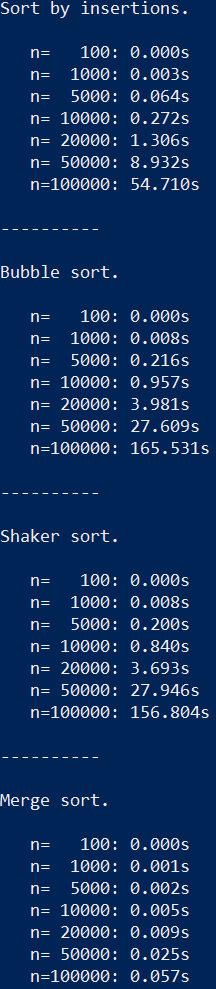
\includegraphics[width=0.25\linewidth]{tests.png}
	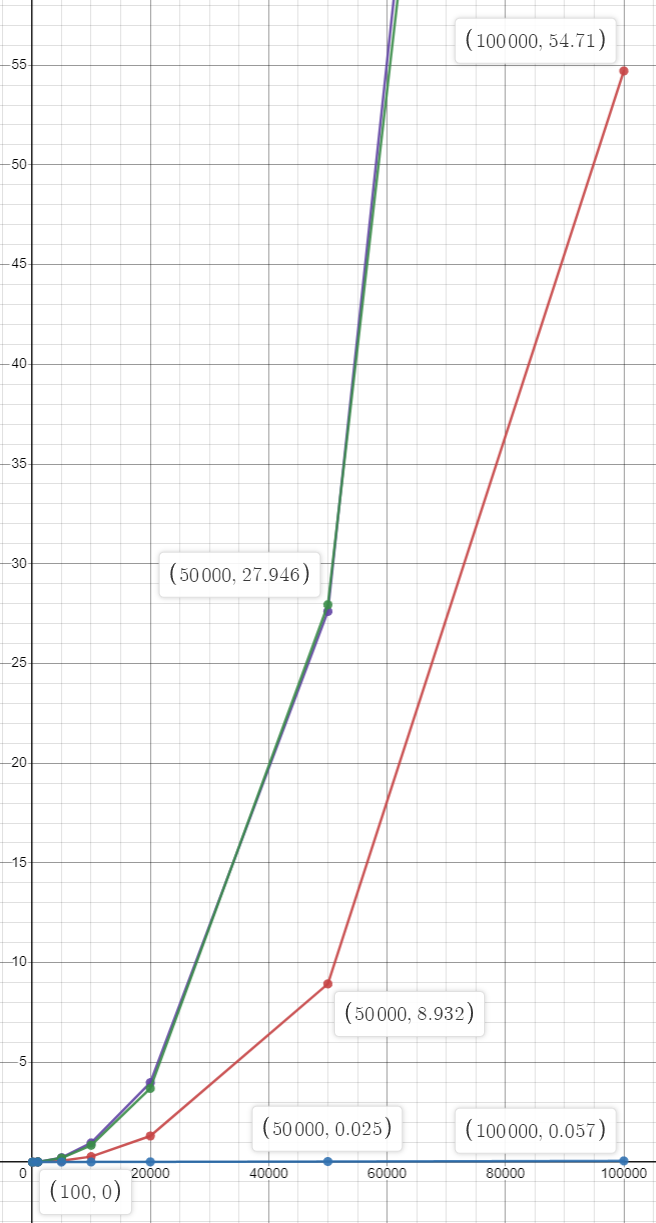
\includegraphics[width=0.75\linewidth]{graphics.png} \newline
	По времени эффективнее всех оказывается сортировка слиянием. Дальше по порядку идут: сортировка вставками, сортировка шейкером, пузырьковая сортировка.
	Естественно, по затратам памяти самой неэффективной оказывается сортировка слиянием, но затраты по памяти полностью компенсируются временными.
	
	\subsection{Тест 2}
	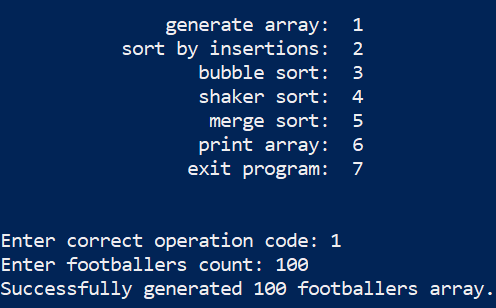
\includegraphics[width=1\linewidth]{test_2.png} \newline
	Успешная генерация массива футболистов соответствующего размера.
	
	\subsection{Тест 3}
	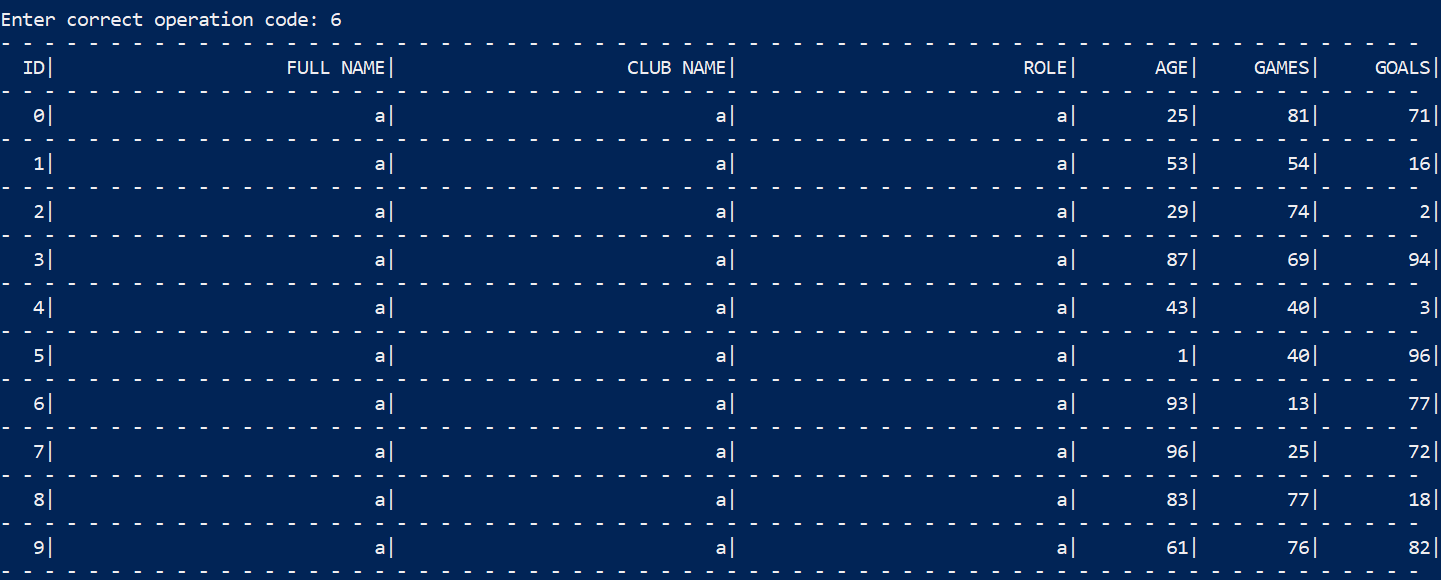
\includegraphics[width=1\linewidth]{test_3.png} \newline
	Успешный вывод массива футболистов соответствующего размера.
	
	\subsection{Тест 4}
	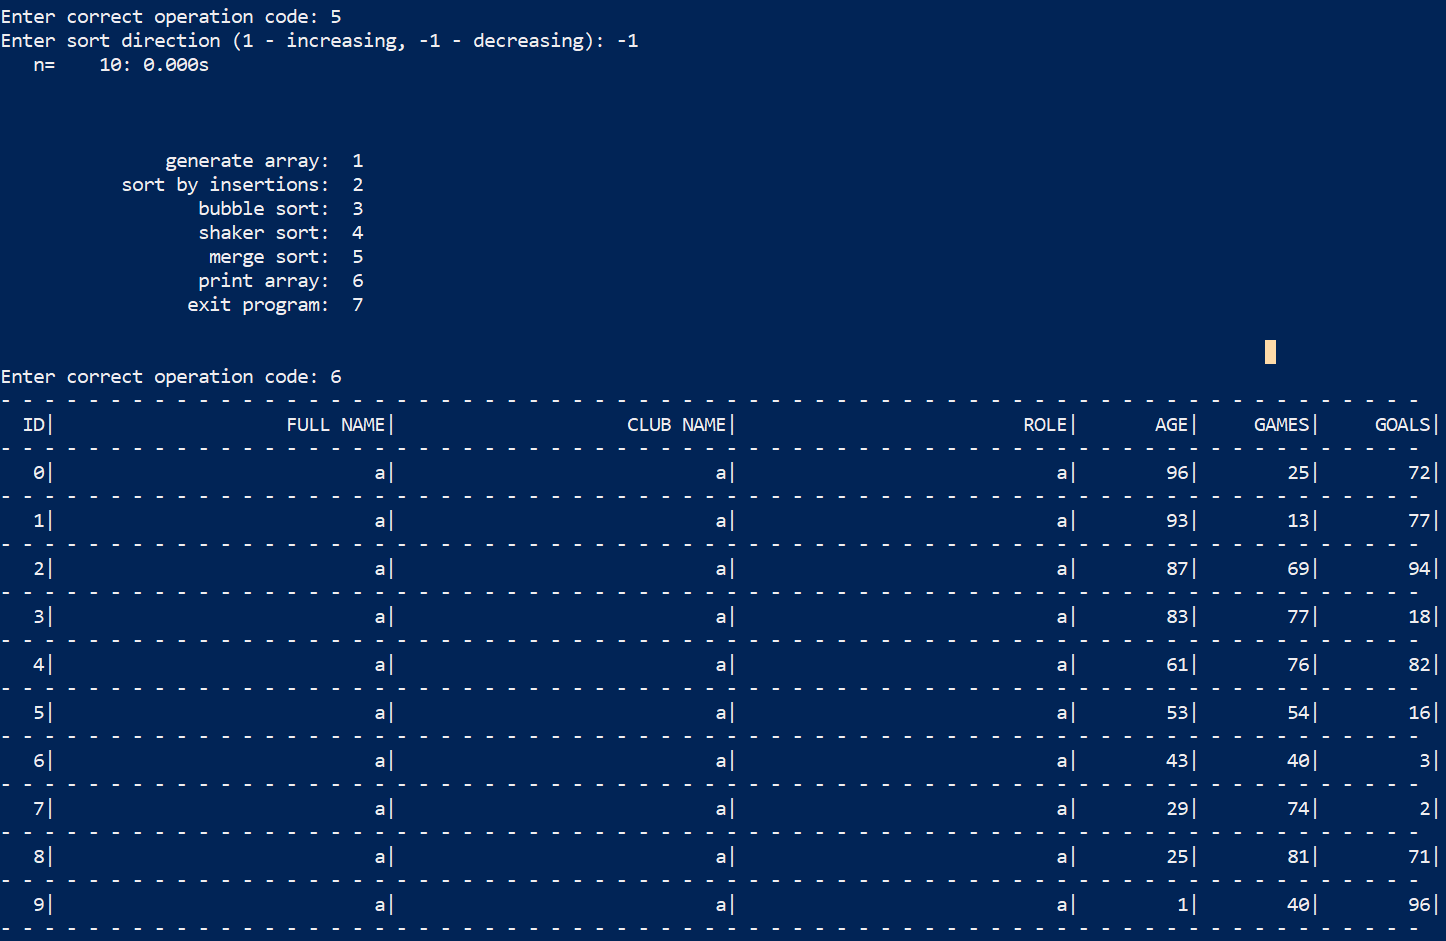
\includegraphics[width=1\linewidth]{test_4.png} \newline
	Успешная сортировка массива футболистов в соответствующем направлении.
	
\end{document}
